\chapter{Recent stuff, title this better.}
\label{ch:kron_taco}

\section{Introduction}
The preceding chapter left me with a few open questions. The analytical cost
models of Chapter~\ref{ch:pact} predicted operation counts accurately, but
operation counts proved a very poor proxy for runtime (perhaps predictably, a memory operation in one context is sometimes orders of magnitudes
slower than a memory operation in another due to caching), and the heterogeneous
per-block pipeline built on them did not outperform a single simple globally
chosen format. Those experiments could show that the models
failed to predict performance, but not exactly why. They also relied on
a small set of synthetic inputs, so they said little about how
the best format combination changes as a matrix grows or as its
structure changes.

This chapter returns to the these unanswered with the upgraded reptest library and a bit more systematic experiment design. Rather than building a more
elaborate selection mechanism first, I asked the more basic question I should have started with. For
sparse$\times$sparse matrix multiplication, how does the best pairing of storage formats vary with matrix structure and scale, and, importantly, what hardware
behavior explain these differences? This question informed the design choices I made below.

\paragraph{Structured inputs.}
Graph adjacency matrices are a common source of sparse matrix inputs, and
Kronecker graphs \cite{kronecker} are a natural family to study. They are
generated from a small 'initiator' matrix by repeated Kronecker products, so
their structure is reproducible while still exhibiting structure commonly associated with real networks.
In addition, the same graph family can be generated at many scales.

\paragraph{Sweeping scale instead of comparing individual graphs.}
Sparse linear algebra benchmarks are often reported as results on a
collection of well-known, common matrices/graphs, typically as one bar per matrix.
Such comparisons can be informative, but they confound size, density, and
structure, and it can be hard to determine where or why performance behavior changes. Because
Kronecker graphs can be generated at successive scales of $k$, each family
can be swept across $k$, producing continuous curves in which crossover
points between formats are visible directly.

\paragraph{Explaining performance with hardware counters.}
Chapter~\ref{ch:reptest} describes the benchmarking library I built, which
reads hardware counters through Linux \texttt{perf} sycalls. In the earlier
experiments, only operation counts and cycle counts were available, and
the gap between them could only be speculated about. In the new experiments, each reptest
measurement also records cache misses, branch mispredictions, page faults
so that differences in runtime between format pairings can be tied to specific observed behavior rather than inferred or guessed.

\paragraph{TACO-generated kernels.}
In Chapter~\ref{ch:pact}, the kernels were rewritten by hand to embed
instrumentation. In this chapter, kernels
are generated by the TACO compiler \cite{taco}, which derives code
for any combination of formats from a single algebraic specification with 'scheduling' commands. This makes
the comparison between formats more even-handed, since every pairing is
produced by the same process. However, it also exposed practical limits of using TACO at scale:
generated code assumed 32-bit sizes in allocation, which fails for most kronecker matrices tested of
roughly $2^{20} \times 2^{20}$ and above. I describe the changes made to support these sizes in Section~\ref{sec:taco-limits}.

\paragraph{Scope.}
I restricted my attention to sparse$\times$sparse products. \note{probably more to say here..}

\paragraph{Blocking.}
\note{TODO: Once these experiments are finished...}

% \paragraph{Contributions.}
% This chapter contributes:
% \begin{enumerate}
%   \item a systematic comparison of sparse format pairings for SpGEMM across
%         [number] Kronecker graph families, each swept over scales
%         $k = [\ldots]$;
%   \item hardware-counter evidence explaining the observed crossovers
%         between formats [fill in once findings are settled];
%   \item a description of the limitations of TACO-generated code at large
%         matrix sizes, and the modifications needed to run past them.
% \end{enumerate}

% \paragraph{Chapter organization.}
% Section~\ref{sec:kron-method} describes the experimental setup,
% Section~\ref{sec:taco-limits} discusses the TACO modifications,
% Section~\ref{sec:kron-results} presents results, and
% Section~\ref{sec:kron-discussion} interprets them in light of the earlier
% chapters.
\section{Taco Limitations}
\note{Oh boy.}

\section{Results}
\note{TODO: Translate notes to academic-speak, also update with most recent figures, also figure out why matplotlib is overlapping the titles...}

% \begin{figure}[t]
%   \centering
%   \includegraphics[width=\linewidth]{figures/taco_bench_altogether.png}
%   \caption{TODO: This needs to be broken up, this is unreadable, probably do the grid based? or perhaps just try letting each sub-figure be its own figure while still having each kronecker to be on the same one... more comparable that way...}
%   \label{fig:taco_altogether}
% \end{figure}

\begin{figure}[t]
  \centering
  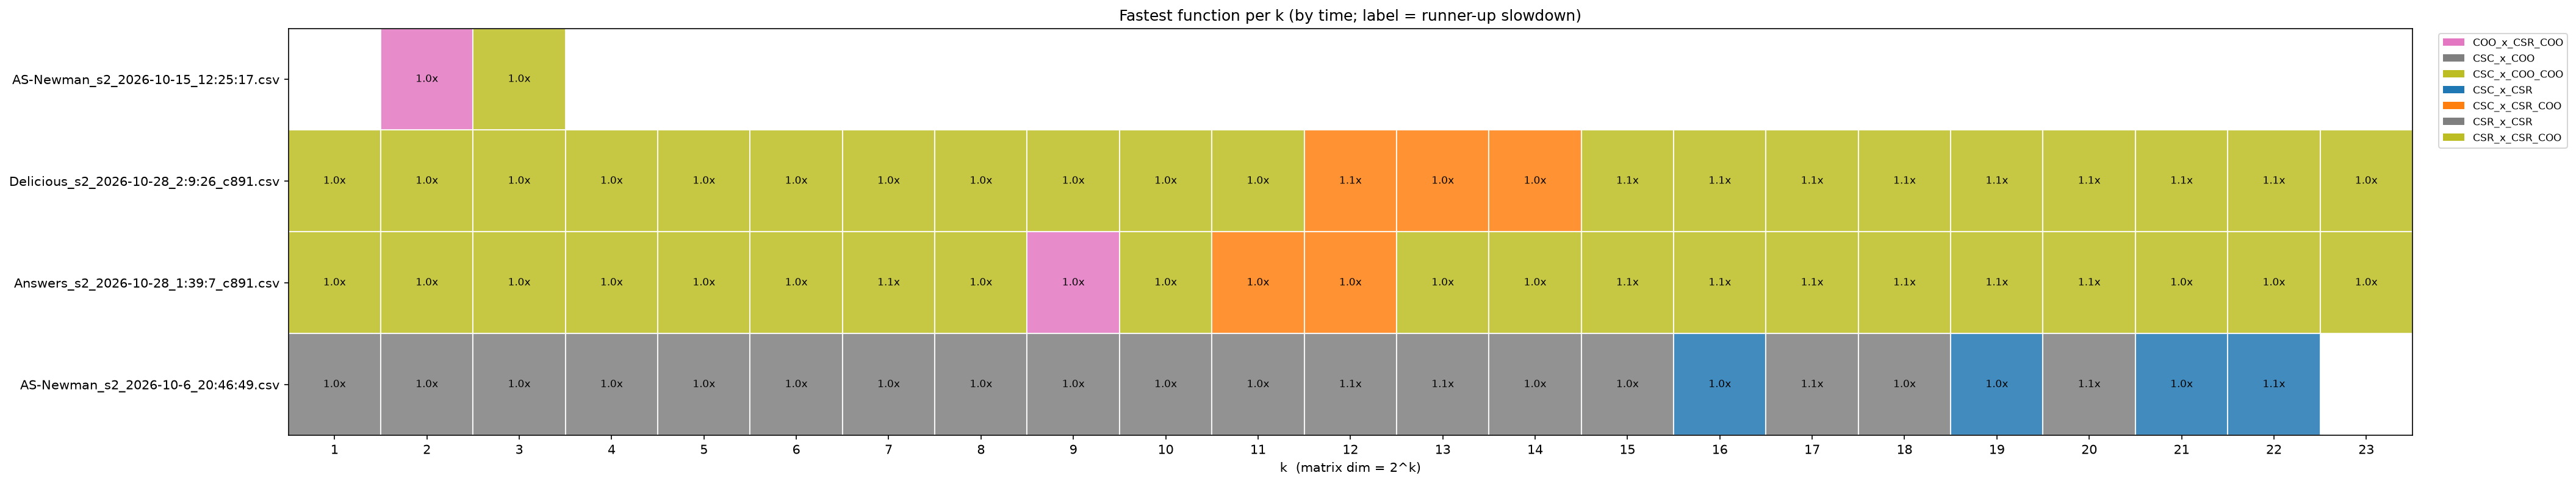
\includegraphics[width=\linewidth]{figures/taco_bench_best_for_k.png}
  \caption{TODO: this one is going to be humongous with all of them. Also need to do this across more than just varying K, again don't want to make the mistake of confounding the difference come from structure when it may just be due to density or size... also need to mention that runner-ups are very, very close in almost all cases.}
  \label{fig:taco_best_for_k}
\end{figure}
